\label{chapter:intro}
We now move away from systems biology and into my research in
classical Density Functional Theory.  \fixme{Is there a nice way to do
this transition smoothly?}


The standard approach in liquid state theory is to model a liquid as a
hard-sphere reference fluid with attractive interactions that are
treated perturbatively~\cite{hansen2006theory}.  Recent advances have
extended these perturbative approaches to inhomogeneous density
distributions---that is, liquid interfaces---through the use of
classical density functional theory (DFT), in which the grand free
energy is found by minimizing a free energy functional of the
density~\cite{jain2007modified, gloor2007prediction,
  gross2009density,
  %felipe2001examination, gloor2002saft,
  %gloor2004accurate, clark2006developing,
  kahl2008modified,
  % yu2002fmt-dft-inhomogeneous-associating,
  %fu2005vapor-liquid-dft, bryk2006density,
  hughes2013classical,
  %segura1998comparison, felipe2001examination,
  %gloor2002saft, gloor2004accurate, fu2005vapor-liquid-dft,
  bryk2006density, clark2006developing, kahl2008modified,
  gross2009density} In the following section I introduce the
  theoretical origins of classical DFT, a basic understanding of which
  is neccesary for anyone looking to work in liquid state theory.

\section{Classical Density Functional Theory}

A classical statistical ensemble is a collection of an arbitrary
number of classical systems of particles that have the same
macroscopic properties and internal restrictions, but have positions
and momenta that are otherwise distributed randomly.  In the canonical
ensemble, the number of particles $N$, the total volume of the system
$V$, and the tempurature $T$ are constant.  In this ensemble the free
energy, defined as $F = U - TS$, where $U$ is the internal energy and
$S$ is the entropy of the system, is at a minimum in thermodynamic
equilibrium. In the grand canonical ensemble, the number of particles
is allowed to vary while $V$, $T$ and the chemical potential $\mu$ are
constant.  In this ensemble it is the grand potential, defined as
$\Omega = F - \mu N$, that is at a minimum in thermodynamic
equilibrium.

In the case of inhomogenous fluids, a treatment of the inhomogenous
external potential $\phi(\rr)$ restricts the positions of the
particles in the system and stands in the place of the volume $V$ in
the thermodynamic equations.  In such a system, a change in the
internal energy is
\begin{align}
  \delta U = T\delta S + \int \rho^{(1)}(\rr)\delta \phi(\rr)d(\rr) + \mu \delta N
\end{align}
where $\rho^{(1)}$ is the 'one particle density'.
$\rho^{(1)}(\rr)d\rr$ is the average number of particles at $\rr$
within a volume $d\rr$.  One can calculate $\rho^{(1)}(\rr)$ by taking
the one-particle limit of the n-particle density of the grand
canonical ensemble,
\begin{align}
  \label{eq:n-particle-density}
  \rho_N^{(n)}(\rr^n)=\frac{1}{\Xi}\sum^{\infty}_{N=n}\frac{exp(N\beta \mu)}{\Lambda^3 (N-n)!} \
  \int exp(-\beta V_N)d\rr^{(N-n)}.
\end{align}
$\rho_N^{(n)}(\rr^n)$ has the general form of a statistical mechanical
probability, with an integration over possible states of Boltzmann
factors divided by the grand canonical partition function,
\begin{align}
  \Xi = \sum_{N=0}^{\infty}\frac{exp(N\beta\mu)}{h^{3N}N!}\int\int exp(\beta \mathcal{H})d\rr^Nd\mathbf{p}^N.
\end{align}
$V_N$ in Eq.~\ref{eq:n-particle-density} is the total interaction
potential between all of the particles in the system, and the spatial
integral is taken over all the potential positions of the particles
\emph{other} than the $n$ particles at positions $\rr^n$.  The
$exp(N\beta \mu)$ term accounts for the chemical potential's
regulation of the average number of particles in the system.  When
implementing density functional theory, one adjusts $\mu$ in order to
restrict the system's average number of particles,
\begin{align}
  \int_{system} \rho_N^{(1)}(\rr)d\rr = \langle N \rangle
\end{align}
to be a desired value.

The probability density, which is closely related to the n-particles
density, is $f_0(\rr^N,\mathbf{p}^N;N)$.
$f_0(\rr^N,\mathbf{p}^N;N)d\rr^N$ is the probability that there are
$N$ particles in the system and that those particles are found within
the infinitesimal range of positions $\rr^N$ and momenta
$\mathbf{p}^N$.  It's definition is
\begin{align}
  \label{eq:prob-density}
  \mathit{f}_0(\rr^N,\mathbf{p}^N;N) = \frac{exp(-\beta(\mathcal{H}-N\mu))}{\Xi}
\end{align}
where $\Xi$ is once again the partition
function.

Classical Density Functional Theory assumes that the Hamiltonian can
be split into linearly combined parts:
\begin{align}\label{eq:hamiltonian}
  \mathcal{H}(\rr^N,\mathbf{p}^N) = K_N(\mathbf{p}^N) + V_N(\rr^N) + \Phi(\rr^N)
\end{align}
The three terms on the right are the kinetic energy, potential
interaction between particles, and external potential, respectively.
The kinetic energy is a function of only the momenta of the particles,
and the two potentials of only their positions.

Substituing this for the Hamiltonian term in Eq.~\ref{eq:prob-density}
and taking the natural logarithm, we have:
\begin{align}
  \label{eq:log-of-f}
  \ln \mathit{f}_0 = \beta\Omega - \beta K_N - \beta V_N - \beta \Phi_N + N\beta \mu
\end{align}
where we have used the relation
\begin{align}
  \Omega = -k_BT\ln\Xi,
\end{align}
which is the basic connection between thermodynamics and statistical
mechanics in the grand canonical ensemble.

Because the external potential $\Phi(\rr)$ and $\mu$ are both constant
and $\rho^{(1)}(\rr)$ is the average ensemble equilibrium density at
$\rr$, the two right most terms are
\begin{align}
  \langle \Phi_N \rangle = \int \rho^{(1)}(\rr)\phi(\rr)d\rr \
  and \
  \langle N\mu \rangle = \mu \int \rho^{(1)}(\rr) d\rr
\end{align}

Using these relations and switching terms around in
Eq.~\ref{eq:log-of-f} results in the equation
\begin{align} \label{eq:intrinsic-free-two}
  \langle K_N + V_N + k_BT \ln \mathit{f}_0 \rangle \
  = \Omega - \int \rho^{(1)}(\rr)\phi(\rr)d\rr + \mu \int \rho^{(1)}(\rr)d\rr
\end{align}

The thermodynamic definition of the grand potential gives us $F =
\Omega + \mu N$.  From this we can see that the right hand side of
Eq.~\ref{eq:intrinsic-free-two} is analougous to the free energy of
the inhomogenous system minus the energy due to the external
potential.  We call this function the 'intrinsic free energy' $\iF$
since it only includes the interaction energy between the particles
within the system:

\begin{align}
  \label{eq:intrinsic-free-three}
  \iF = \Omega - \int \rho^{(1)}(\rr)\phi(\rr)d\rr + \mu \int \rho^{(1)}(\rr)d\rr \
  = \langle K_N + V_N + k_BT \ln \mathit{f}_0 \rangle
\end{align}

It can be shown that for a given $\mu$, $T$, and defined function
$V_N$ describing the potential interaction between particles, there is
a one-to-one relation between the external potential function and the
equilibrium density profile $\rho^{(1)}$ at thermodynamic equilibrium.
The grand canonical density function $f_0$ (Eq.~\ref{eq:prob-density})
for a given function $V_N$, $\mu$, and $T$ is a function of only the
external potential, so as a result it is completely determined by
$\rho^{(1)}$.  $V_N$ is also wholly determined by $\rho^{(1)}$ and
$K_N$ is determined by tempurature.  Thus the right hand side of
Eq.~\ref{eq:intrinsic-free-three} is a function of only the external
potential and therefore also of only $\rho^{(1)}$, which means that
for a given $\mu$, $T$, and defined function $V_N$, $\iF$ is wholly
determined by $\rho^{(1)}$.

Thanks to all of this, we can write
\begin{align}
  \Omega_{\phi}[n] = \iF[n] + \int n(\rr)\phi(\rr)d\rr - \mu\int n(\rr)d\rr
\end{align}
where $n(\rr)$ is a density profile that we will adjust systematically
in order to minimize $\Omega_{\phi}[n]$.  When $\Omega_{\phi}[n]$ is
minimized, it becomes the minimized grand potential of the system, and
the density profile $n(\rr)$ of the system is the density profile in
thermodynamic equilibrium, $\rho^{(1)}$.  It is finding this density
profile in thermodynamic equilibrium, and then the properties that can
be derived from it, that is the ultimate goal of Classical Density
Functional Theory.  Throughout the rest of this dissertation I will be
using $n(\rr)$ to refer to the particle density of the system, and the
reader should understand that it is a function that is meant to be
adjusted in order to minimize the grand potential energy function.

We begin the process of Classical Density Functional Theory by
designing the functional form of the intrinisic free energy $\iF$.
This is the major theoretical part of the process.  We then decide
upon an external potential $\phi(\rr)$ that defines the external
restrictions of the system, set the tempurature $T$ and chemical
potential $\mu$, and systematically adjust the density profile until
we have found the global minimum of this grand potential.  I won't
discuss the process of finding the density profile that minimizes the
grand potential in this dissertation, primarily because the algorithms
that do this were all in place before I joined the lab!  My work is
centered around the first part of the process, namely constructing the
functional form of $\iF$.



\clearpage
\newpage



\section{Introduction to SAFT and explanation of first free energy term}

Work on Classical Density Functional Theory for inhomogeneous fluids
involves creating the intrinsic free energy functional of the density
profile, $\iF[n]$.  This is comprised of a sum of terms that
individually address different conceptual aspects of the system.
Terms that treat different types of interaction between particles are
added to a term that describes the reference system.

The free energy functional that we use in our work is one of a widely
used family of models in the development of classical density
functionals called Statistical Associating Fluid Theory
(SAFT)~\cite{chapman1989saft}.  SAFT is a theory based on a model of
hard spheres with weak dispersion interactions and hydrogen-bonding
association sites, which has been used to accurately model the
equations of state of both pure fluids and mixtures over a wide range
of temperatures and pressures~\cite{muller2001molecular,
tan2008recent}. We will discuss the concept of hard spheres in detail
in following sections.

A SAFT functional is broken into the following terms:
\begin{align}
  \iF_{SAFT} = F_{ideal} + F_{hard sphere} + F_{dispersion} + F_{association}
\end{align}
We will discuss the meaning of these terms below in much more detail,
but write it down now to illustrate the general structure of the total
functional.


Although we work specifically with the SAFT functionals in current
development, our contributions described in the next chapters are
applicable to many different types of fluid functionals.  The next
chapter details a functional that we've created, the distribution
function at contact $g_\sigma(\rr)$, which treats correlations between
particles within a system, while the following chapter discusses it's
use within a specific SAFT functional and it's effect upon that
functional's results.  The chapter after that introduces another
function, the pair distribution function $g^{(2)}_{HS}(\rr_1,\rr_2)$,
that is closely related to the first.  It's important for the reader
to recognize that while we discuss these functions in terms of their
place within the SAFT free energy, they and their conceptual founding
are useful to other Classical Density Functional Theories.



The first two terms, $F_{ideal}$ and $F_{hard~sphere}$, are typically
thought of as the functional's reference system terms.  The
$F_{ideal}$ is ubiquitous, and treats particles that have no
interactions between them.  While the $F_{hard~sphere}$ term does
treat particle interactions, the type of interaction it treats is so
basic and simple that this term is also seen as a reference term and
is incorporated into many very different functionals.  I give a
detailed introduction to the particular functional that we use for the
$F_{hard~sphere}$ term below (that of the White Bear free energy),
because while we don't actually modify it in our implementation of
inhomogenous SAFT, we do draw heavily from its ideas when creating our
functions.  The rest of the terms in $\iF$ address different types of
interactions between particles.  SAFT itself departs from other
theories in these last two terms.  In inhomogenous fluids, each one of
these terms is itself a functional of the density profile.


The first term in the SAFT functional is the ideal free energy term
$F_{ideal}$, and it treats a system of particles that do not interact
with eachother.  This is an obvious place to start if one is to build
the description of particle interaction terms upon a reference system.
It's lack of interaction actually causes this term to be the only one
that we can construct exactly, with no approximations.  To see why, we
point out that a system of non-interacting particles is able to
satisfy what is usually called the the local density approximation
(although we shouldn't call it this here because for non-interacting
particles it's not an approximation!)  The idea is that the free
energy functional can be written as an integral of a completely local
function of the density profile:
\begin{align}
  \iF_{local~density}[n] = \int f(n(\rr)) d\rr
\end{align}
where $f(n(\rr))$ is the free energy per unit volume of a homogenoues
fluid at a density $n(\rr)$.  In essence, each bit of volume becomes
it's own thermodynamic system, with a free energy equal that of a
homogenous density of particles at the local density, and the free
energies from all the bits of volume are added up to get the total.
The construction neglects any interaction between the particles, so
that any spatial variation in the density will be due entirely to the
varying external potential.  As an approximation for interacting
fluids, it does in fact apply to external potentials that modulate the
density slowly over space, much more slowly than correlation lengths.
It has thus been used in the past to construct entire intrinsic free
energy functionals beyond the reference $F_{ideal}$ term (cite).  It
breaks breaks down rather quickly, however, near hard walls for
interacting systems, where often the spheres will stack up in 'layers'
(should see some figure) and the local densities become greater than
bulk freezing densities (cite).

However, $F_{ideal}$ can be constructed exactly in this integral of
local density fashion, so all we need to do is integrate the free
energy of an ideal homogenous system at the local density.  Going back
to basic thermodynamics and statistical mechanics, we have:
\begin{align}
  F = -k_BT \ln Q_N = -k_BT \ln (\frac{V}{N!\Lambda^3})
\end{align}
where $Q_N$ is the partition function and $\Lambda$ is de Broglie
thermal wavelength.  Using th Stirling approximation for $N!$, we have
\begin{align}
F^{id} = Nk_BT(\ln \Lambda^3 \rho - 1))
\end{align}
Taking this as the free energy per unit volume and integrating, we
have
\begin{align}
  F_{ideal}[n] = \frac{1}{\beta}\int d\rr n(\rr)(\ln (\Lambda^3 n(\rr))-1)
\end{align}
This will be our reference $F_{ideal}$ term, as is common within
Clasical Density Functional Theory.

\clearpage
\newpage

\section{Virial Equation, Mayer functions, and the Carnahan Starling Equation}

The second term in the SAFT intrinsic free energy functional,
$F_{hard~sphere}$, is generally refered to as a reference term and the
specific functional that we use for this term is also used in many
other density functional theories.  I'll introduce the functional and
the theory behind it in some detail in the next section because it is
so widely used and, more importantly, because an understanding of the
ideas involved is neccesary for an understanding of our own work.
Before describing the term itself, however, I'll explain in this
section some important things that lead up to this theory, namely the
Virial equation, Mayer functions, and the Carnahan Starling Equation.

The Virial Equation applies to homogeneous fluids.  It equates a
thermodynamic, intensive quantity (likes the pressure) to an expansion
of the homogeneous density of the fluid.  It's standard form is
\begin{align}
  \label{eq:virial-expansion}
  \frac{\beta P}{\rho} = 1 + \sum_{i=1}^{\infty}\beta_i\eta^i.
\end{align}
where
\begin{align}
  \eta = \frac{\pi \rho \sigma^3}{6}
\end{align}
is the 'packing fraction'.  $\sigma$ here is the diameter of the
spherical particles of the fluid.  The packing fraction is really just
a more convenient way to refer to the density, where we give each
particle the volume of a sphere and think in terms of how much volume
is taken up by particles as opposed to how many there are.  We use it
extensively throughout our work.

The expansion of Eq.~\ref{eq:virial-expansion} comes out of a
formulation of the partition function that is most often expressed as
a series of diagrams that have well defined rules of construction.  I
won't explain the diagrams or their rules here, but
Figure(\fixme{should I show some diagrams here?  Where should I get
them from?  Would it be okay to just use inkscape or something to do
it myself?}) shows an example so that if the reader sees them
somewhere she'll know what they are.  A single term (or diagram) in
this expansion of the partition function is in fact a spatial integral
of particle densities multiplied by a number of what are called Mayer
Functions.  I'll give a loose outline of an explanation here, since a
basic idea of where this expansion comes from should be useful to the
reader.  The derivation starts with the partition function:
\begin{align}
  \Xi &= \sum_{N=0}^{\infty}\frac{exp(N\beta\mu)}{h^{3N}N!}\int...\int exp(-\beta \mathcal{H})d\rr^Nd\mathbf{p}^N \\
  &=\sum_{N=0}^{\infty}\frac{exp(N\beta\mu)}{h^{3N}N!}\int...\int exp(-\beta (V_N + \phi(\rr))d\rr^Nd\mathbf{p}^N
\end{align}
where $V_N$ is the interaction potential between all the particles in
the system and $\phi(\rr)$ is the external potential.  If the the
interaction potential can be written as a summation of pairwise
superposable interactions, i.e.
\begin{align}
  V_N = \sum_{i<j}^{all~particles} v(i,j)
\end{align}
 than the partition function can be written as
\begin{align}
  \Xi = \sum_{N=0}^{\infty}\frac{1}{N!}\int... \int \left(\overset{N}{\underset{i<j}{\Pi}} f(i,j)\right)
  \left( \overset{N}{\underset{i=1}{\Pi}} \frac{exp(\beta (\mu - \phi(\rr)))}{\Lambda^3}\right)d\rr^N
\end{align}
where $f(i,j)=exp(-\beta v(i,j))$ is the Mayer function between two
particles.  With the help of the diagrams, one can take the natural
logarithm of the partition function to get the grand potential, and
then derivatives to find what are called direct correlation functions
(which I won't explain here). The use of an identity yields a
relationship between the chemical potential and the density,
\begin{align}
  \beta \mu = \beta \mu^{id} - \sum_{i=1}^{\infty}\beta_i\rho^i.
\end{align}
Then the use of the relation from thermodynamics,
\begin{align}
  \left(\frac{\partial P}{\partial \rho}\right)_T \
  = \rho \left(\frac{\partial \mu}{\partial \rho}\right)_T,
\end{align}
allows one to express the pressure as
\begin{align}
  \frac{\beta P}{\rho} = 1 + \sum_{i=1}^{\infty}\beta_i\eta^i
\end{align}
where
\begin{align}
  \label{eq:virial-coeff}
  \beta_i = (\frac{6}{\pi \sigma^3})^i B_{i+1}.
\end{align}

The virial formulation of thermodynamic properties is useful, but it
requires an expansion of coeffients, which can be a nuisance
computationally.  Carnahan and
Starling~\cite{carnahan1969equation,mansoori1971equilibrium} were able
to develop a rule for coefficient generation that approximates
Eq.~\ref{eq:virial-coeff}, but that results in integers that one can
use to make a geometric series.  Written in its analytic form, this
series is a simple, easy to use, and accurate approximation of the
pressure in a homogenous fluid as a function of density (or packing
fraction $\eta$):
\begin{align}
  \frac{\beta P}{\rho}=\frac{1+\eta+\eta^2-\eta^3}{(1-\eta)^3}
\end{align}
It also yields the free energy in the form
\begin{align}
  \frac{\beta F^{ex}}{N}=\frac{\eta(4-3\eta)}{(1-\eta)^2}.
\end{align}
This equation is specifically very successful in predicting the
pressure of the homogenous hard sphere fluid at different densities.



\section{$F_{hard~sphere}$, Fundemental Meaure Theory, and White Bear}

\fixme{White Bear uses MCSL equation of state, which is the generalization to
the multi component mixture of hard spheres of the Carnahan-Starling
equation of state.}

We now return to analyzing the terms that make up the SAFT free energy:
\begin{align}
  \iF_{SAFT} = F_{ideal} + F_{hard~sphere} +  F_{dispersion} + F_{association}.
\end{align}

Remember that the $F_{ideal}$ term treats particles that do not
interact with one another.  In fact,
this one term addresses any aspect of the system that is
non-interactive, in the sense that every other term in $\iF_{SAFT}$ is
designed to specifically deal with a different type of potential
interaction among the particles.  Thus, $F_{ideal}$ is in a sense the
most basic reference term in the system.  However, as I've stated
above, the second term, $F_{hard~sphere}$, which I will describe here,
is also considered to be a reference system.

The potential interaction it describes is based on the fact that every
particle has at it's core a 'hard-core' repulsion to any other
particle.  In other words, as two particles approach each other in
space, there is a sudden, sharp spike in potential that prevents the
two particles from 'overlapping'.  The forces here can be complicated,
deriving from nuclear forces and the exclusion principle, but our
classical theories seek to approximate these in simple ways.

The hard sphere potential interaction is characterised by an
impenetrable spherical volume that is centered at a particles'
position.  The potential between two of these hard spheres
discontinuously jumps from zero to infinity when the spheres are a
distance apart that is equal to their combined radii:
\begin{align}
  v(r) &= \infty,~~ r < r_A + r_B \\
  &= 0,~~ r > r_A + r_B
\end{align}
where $r$ is the distance between the two particles, and $r_A$ and
$r_B$ are the radii of the two particles.  This hard sphere potential
that we use is not the only commonly used method for treating the
hard-core repulsion between particles.  The Leonard-Jones potential,
for example, another widely used potential energy description,
approximates the repulsion with a positive term porportional to
$\frac{1}{r^{12}}$


After deciding upon this form for the potential, one must turn to the
much more difficult step of designing an appropriate free energy
functional.  One of the first methods by which people attempted to
deal with these interactions, which is actually not limited to hard
spheres, was to modify the form of the local density approximation
free energy discussed above,
\begin{align}
  F_{local~density}[n] = \int f(n(\rr)) d\rr
\end{align}
to incorporate information about the particle densities immediately
surrounding each point.  They did this by redefining the density at
each point to be a convolution of the surrounding density with a
weighting function:
\begin{align}
  \label{eq:convolution-of-density}
  \bar{n}(\rr) = \int w(|\rr-\rr'|) n(\rr') d\rr'
\end{align}
and then using a function of this modified density as a weighting
function in the local density approximation formulation of the free
energy:
\begin{align}
  \iF[n] = \int \frac{f^{ex}(\bar{n}(\rr))}{\bar{n}(\rr)} n(\rr) d\rr
\end{align}
Eq.~\ref{eq:convolution-of-density} allows one to shape the nature of
the interaction indirectly, by changing the structure of the weighting
function.  For example, if one were to choose for the weighting
function the step function $\Theta(|\rr-\rr'|)$, than the modified
density would incorporate in an equal way all the density within a
sphere surrounding the particle.  A functional constructed in this way
would be a very oversimplified example of a weighted density
approximation.  Practical theories formulated in this manner become
very complicated.  We introduce it here so that the reader knows what
it is and also because the central idea described by
Eq.~\ref{eq:convolution-of-density} is used in Fundemental Measure
Theory, which we will now describe, as well.

Fundamental Measure Theory (FMT), created by Rosenfeld in
1989 \cite{rosenfeld1989free,rosenfeld1990free}, also defines the free
energy in terms of a series of convolutions of densities, but it is a
considerable departure from the weighted density approximation
theories.  It is based on an involved derivation worked out by Perkis
and Yevik of an equation of state for a homogeneous fluid.  Like the
derivation of the Virial Expansion and Carnahan-Starling Equation
discussed above, this derivation also dealt with correlation functions
and ultimately expressed thermodynamic properties in terms of
homogeneous density.  Rosenfeld compared this theory with the
derivations of another theory call Scaled Particle Theory, which once
again I will not explain but will say that it has to do conceptually
with a system of spheres and a growing cavity in which they are not
allowed to go.  He recognized that the density sides of the
Perkis-Yevick equations can be reformulated in terms of densities and
functions constructed to describe the geometric properties of spheres.
Rosenfeld then discovered that for inhomogeneous systems, he could
write down the intrinsic free energy in terms of convolutions of
densities with these spherical functions in such a way that the
Percis-Yevik correlation equations were reproduced in the limit of
homogeneous density.  The derivation is certainly an involved (and
brilliant) one, and there is actually another derivation to get to the
same place introduced by Tarazona and
Rosenfeld~\cite{tarazona1997,tarazona1999free,tarazona2000,tarazona2002fundamental}
that is thought by some to be more elegant.  However I don't use any
ideas that are directly pulled from these derivations in my work,
besides those that can be taken from the general characteristics
(spherical nature) of the resulting Free Energy functional.

The result of all this is an intrinsic free energy which has the form:
\begin{align}
  \label{eq:F-FMT-form}
  \iF_{hard~sphere}[n] = \int \Phi({n_i(\rr)})d\rr
\end{align}
The integrand $\Phi$ here is a local function of $n_i(\rr)$, which are
the non-local convolutions of density with sphere-like weighting
functions discussed above.  In FMT they are referred to as
'fundamental measures'.  They are defined as:
\begin{align}
  n_3(\rr) &= \int n(\rr') \Theta(\sigma/2 -\left|\rr - \rr'\right|)
  d\rr' \label{eq:FMn3} \\
  n_2(\rr) &= \int n(\rr') \delta(\sigma/2 -\left|\rr - \rr'\right|) d\rr' \\
  \mathbf{n}_{2V}(\rr) &= \int n(\rr') \delta(\sigma/2 -\left|\rr - \rr'\right|) \frac{\rr-\rr'}{|\rr-\rr'|}d\rr'
\end{align}
\begin{align}
  \mathbf{n}_{V1} = \frac{\mathbf{n}_{V2}}{2\pi \sigma}, \quad
  n_1 &= \frac{n_2}{2\pi \sigma} , \quad
  n_0 = \frac{n_2}{\pi \sigma^2} \label{eq:FMrest}
\end{align}
We can see the spherical nature of the theory by inspecting the $n_i$.
The $n_3(\rr)$ weighting function is a step function that is designed
so that the density is integrated over the volume of a sphere of
radius $\sigma/2$, but will make no contributions outside of this
sphere.  $n_2$ only allows for integration of densities on the surface
of a sphere, but incorporates no density within or outside of it.
$n_{2V}$ is a vector version of $n_2$, and the others are different
versions of the same, modified to have different units.

The form of $\Phi({n_i(\rr)})$ is restricted to a certain extent by
dimensional analysis (the units of each term have to be right!)
throughout the derivation, but even given this the theory allows for a
certain amount of freedom in it's design.  Since his derivation of FMT
was originally based on concepts in the Perkis-Yevik derivation of the
equation of state, Rosenfeld constructed the form of his functional so
that in the limit of homogeneous density, the free energy of the
system approaches that given by the Perkis-Yevik equation of state.

While the theory has been a resounding
  success \cite{rosenfeld1989free,rosenfeld1990free,rosenfeld1997fundamental},
  the use of the Perkis-Yevik equation of state as the underlying,
  homogeneous limit equation causes problems.  The construction of FMT
  obeys a theorem called the 'contact value theorem,' which states
  that the pressure at a wall is equal to the temperature multiplied
  by the density in contact with that wall, $p=kTn_{contact}$. This
  theorem is very important in our own work, so I'll discuss it in
  detail below.  I mention it here though because for the hard sphere
  fluid, the Perkis-Yevik equation predicts a pressure that is too
  high as bulk freezing tempuratures are approached.  It consequently
  overestimates the density at contact at these tempuratures.  This is
  problematic, since much of the reason we use classical density
  functional theory in analyzing inhomogeneous fluids in the first
  place is to estimate what happens at walls!

In 2002 Roth et al addressed this issue in their version of FMT which
they named 'White Bear'\cite{roth2002whitebear,hansen2006density},
anecdotally after a pub that they frequented while writing the theory.
They keep the same general form of Rosenfeld's FMT but adjust it so
that in the limit of homogeneous density it's free energy approaches
that of the Mansoori-Carnahan-Starling-Leland equation, a modified
version of the Carnahan-Starling equation of state, which we discussed
above and which we use directly in our own work.  The
Carnahan-Starling is more accurate in limiting cases than the
Perkis-Yevik, so the White Bear hard-sphere free energy functional,
$F_{hard~sphere}$, is overall a more accurate one.  It is therefore
the hard sphere free energy reference system that we choose to use in
our own work.

Below is the entire energy functional written in terms of the
fundamental measure, $n_i(\rr)$:
\begin{equation}
F_\textit{hard~sphere}[n] = k_B T \int \left(\Phi_1(\rr) + \Phi_2(\rr) + \Phi_3(\rr)\right) d\rr \; ,
\end{equation}
with integrands
\begin{align}
\Phi_1 &= -n_0 \ln\left( 1 - n_3\right) \label{eq:Phi1}\\
\Phi_2 &= \frac{n_1 n_2 - \mathbf{n}_{V1} \cdot\mathbf{n}_{V2}}{1-n_3} \\
\Phi_3 &= (n_2^3 - 3 n_2 \mathbf{n}_{V2} \cdot \mathbf{n}_{V2}) \frac{
  n_3 + (1-n_3)^2 \ln(1-n_3)
}{
  36\pi n_3^2\left( 1 - n_3 \right)^2
} , \label{eq:Phi3}
\end{align}

\clearpage
\newpage

\section{Contact Value Theorem}
\begin{figure}
  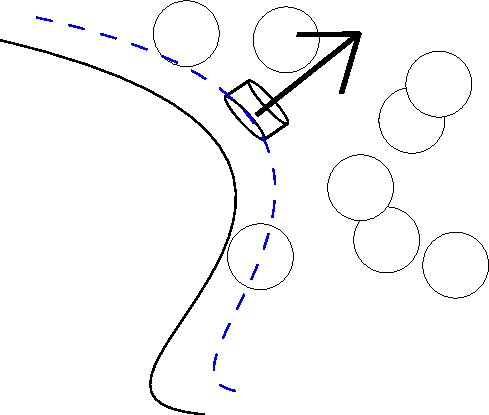
\includegraphics[width=5cm]{contact_one}
  \label{cartoon:bit-of-wall}
\end{figure}

The contact value theorem is used directly in our own work and a
conceptual understanding of its origin will aid in the conceptual
understanding of the functions that we've created.  A derivation of it
is both justified and sort of awesome, so I dedicate this section to
it.

We start by considering a thermodynamic system of a fixed number of
particles.  The thermodynamic equations are:
\begin{align}
F &= U - TS \\
dU &= TdS -pdV \\
dF &= dU - TdS - SdT = -SdT - pdV.
\end{align}
The volume of our system will be fixed except for a tiny
(infinitesimally small) protrusion into it, jutting out from the wall,
illustrated in Figure~\ref{cartoon:bit-of-wall}.  We will allow the protrusion to
either stick out or not, allowing the wall to either be flat and
smooth there or protruding.  We'll call the free energy in the two
different scenarios $F_{flat}$ and $F_{out}$, and investigate the
difference between them, or in other words what happens as the system
loses the bit of volume, dV.  The partition functions for these
scenarios are
\begin{align}
Z_{flat} &= \int_V... \int_V exp(-\phi \{\rr^N \})d\rr^N \\
Z_{out} &=  \int_{V-dV}... \int_{V-dV} exp(-\phi \{\rr^N \})d\rr^N
\end{align}
where $\phi \{\rr^N \}$ is the interaction energy between all the
particles and where we have ignored the kinetic energy terms, since in
both systems, which are at the same tempurature, these will be the
same \fixme{is this definitely true?}, and will later cancel out.  We
would like to write $Z_{flat}$ in terms of $Z_{out}$, so we'll
spatially break up the $Z_{flat}$ intagral.  The first term will
integrate over the same volume as $Z_{out}$.  The next set of terms
will treat the integration for one particle within the bit of volume,
interacting with all the other particles outside of the volume.  The
terms after that will integrate for two of the particles within the
bit of volume and all the remaining particles in the rest of the
volume.  The series will continue on in this fashion, with three
particles in the volume, then four, etc.:
\begin{align}
Z_{flat} = &\int_{V-dV}... \int_{V-dV} exp(-\phi \{\rr^N \})d\rr^N \notag \\
+ &\int_V... \int_V \int_{dV} exp(-\phi \{ \rr^N \})d\rr^N \
+ \int_V ... \int_{dV} \int_V exp(-\phi \{ \rr^N \})d\rr^N ... \notag \\
+ &\int_V... \int_{V}\int_{dV} \int_{dV} exp(-\phi \{\rr^N \})d\rr^N \
+ \int_V... \int_{dV}\int_V \int_{dV} exp(-\phi \{\rr^N \})d\rr^N ...
\end{align}
The term on the first line is just $Z_{out}$.  Looking at the next set
of terms, becuase every particle is identical it doesn't matter which
of them is within the little bit of volume.  Every one of these terms
will be the same, so they can be replaced by one of them multiplied by
$N$.  We will throw away the terms that are of higher order in $dV$,
and there are two arguments that allow us to do this.  The simplest
one is that $dV$ is small, and so terms with two $dV$s multiplied
together will be smaller.  One must be careful with this, however,
because the integration is really of the boltzmann factor over these
volumes.  If the interaction potential between the particles is
constructed so that they are highly attracted to eachother, than a
state in which there are two particles in the bit of volume can have
the same order of magnitude probability as the one in which there is
just one.  In this case we would not be able to say for certain that
these terms are so much smaller than the order one $dV$ terms that we
could reasonably ignore them. Thus the validity of the derivation
depends upon the size of the smallest measurement one can make along
the wall, and the nature of the attractive potential between the
particles.  In our case we deal with an interaction between hard
spheres, which simply exclude other spheres from being too close to
them.  Thus it's reasonable for us to imagine that if there is one
hard sphere in the bit of volume, than there is only the one, and any
terms that address the situation in which there are two in the bit of
volume can be ignored.  After applying these arguments we have:
\begin{align}
  \label{eq:zflat}
  Z_{flat} = Z_{out} + N \int_V... \int_V \int_{dV} exp(-\phi \{ \rr^N \})d\rr^N
\end{align}

Now we consider the statistical mechanical definition of the particle
density,
\begin{align}
  %%n(\rr) &= \frac{N \int_V... \int_V exp(-\phi \{ \rr^N \})d\rr^{N-1}}{\int_V... \int_V exp(-\phi \{ \rr^N \})d\rr^N} \\
  n(\rr) = \frac{N \int_V... \int_V exp(-\phi \{ \rr^N \})d\rr^{N-1}}{Z_{flat}}
\end{align}
Which is the sum of the boltzmann factors of all the states for which
a particle is at position $\rr$, divided by the partition function for
the system.  Comparing this with the right-most term in the
Eq.~\ref{eq:zflat} we see that:
\begin{align}
 N \int_V... \int_V \int_{dV} exp(-\phi \{ \rr^N \})d\rr^N  &= Z_{flat} \int_{dV} n(\rr) d\rr
 &\approx Z_{flat} n(\rr)dV
\end{align}
where on the right we make the approximation that because the volume
is small $n(\rr)$ is constant over it.
Thus we have
\begin{align}
Z_{flat} = Z_{out} + Z_{flat} n(\rr)dV \\
Z_{out} = Z_{flat} (1-n(\rr)dV)
\end{align}

Considering the change in the free energy when the system goes from a
flattened wall to a wall with a tiny protrusion, we have
\begin{align}
  dF = F_{out} - F_{flat} &= -kT \ln \left( \frac{Z_{out}}{Z_{flat}} \right) \notag \\
  &= -kT \ln \left( \frac{Z_{flat} (1-n(\rr)dV)}{Z_{flat}} \right) \notag \\
  &= -kT \ln \left( 1-n(\rr)dV \right) \notag \\
  &= kTn(\rr)dV
\end{align}
Then relating back to thermodynamics:
\begin{align}
  pdV &= dF = ktn(\rr)dV \\
  \label{eq:contact-value-theorem}
  p &= ktn(\rr)
\end{align}
Eq.~\ref{eq:contact-value-theorem} is the standard formulation of the
contact value theorem.


%% Another equation for the particle density is:
%% \begin{align}
%% n(\rr) = \frac{\delta \iF}{\delta V_{ext}}
%% \end{align}

\clearpage
\newpage

\section{Remaining terms in SAFT}

Going back to the terms in the overall SAFT free energy functional,
\begin{align}
  \iF_{SAFT} = F_{ideal} + F_{hard~sphere} +  F_{dispersion} + F_{association},
\end{align}
we come to introducing the last two terms.  These are actually the
only terms in which the functions that we've created show up, but
ironically I'll spend the least amount of time introducing them.  This
is because while the functions that we've created are included in
them, they could also be included in entirely different, non-SAFT
classical density functional theories, and their construction is
dependent on the concepts associated with the preceding terms, not of
$F_{dispersion}$ and $F_{association}$. The chain term describes the
chain formation energy in polymeric fluids, while the association term
describes the effects of hydrogen bonding, both of which can be large.

\clearpage
\newpage

\section{The convolution theorem}

Lastly within this introduction I will introduce a theorem, the
convolution theorem, that is a sort of important side note to the rest
of this text, primarily for the benefit of any new grad students that
might be entering this line of research in the future.  This theorem
motivates our preference of using density convolutions within our
functionals.

One of the largest advantages to using Fundamental
Measure Theory, and one that is not immediately obvious, is that the
convolutions that combine to construct the functional allow for very
efficient computation.  This is not very intuitive, since an integral
of a convolution integral must integrate over two dimensions, e.g.
\begin{align}
\int(f\ast g)(\xx)d\xx = \int \int f(\yy)g(\xx-\yy)d\yy d\xx
\end{align}
so that it may seem that the size of the computation would scale as
$N^2$, where $N$ is the size of the system.  It is true that in the
case of FMT, the weighting functions cut off the integrals at the size
on the order of a sphere of particle radius, but this can still be a
large enough volume so that a double integral for which one of the
volumes is this size and the other is the size of the whole system
would be too costly for practical computation.  FMT is saved, however,
by what is called the Convolution Theorem.  The Convolution Theorem
states that when one takes the Fourier Transform on a spatial
convolution of two functions (a double integral in space), the result
is two separate integrals over k-space that are simply multiplied
together:
\begin{align}
\hat{h}(\kk) = \hat{f}(\kk)\hat{g}(\kk)
\end{align}

When minimizing our functional, after
taking a Fourier Transform of the convolutions, we have merely to
integrate once over the one variable $\kk$.  Wait!  You may say.  This
is a cheat, since the Fourier Transform is itself an integral, so at
the end of the day we're still performing two integrals.  This would
be true if it were not for the computational technique known as Fast
Fourier Transforms, developed by (cite).  I won't explain how it works
here, but it's effect is to perform the transform, which would
normally have a computational cost on the order of N, with a
computational cost on the order of $\ln N$ instead.  Thus, when we
Fourier Transform the convolutions in the functional and proceed to
take the single integral over the result (in k-space), the
computational cost scales as $N \ln N$.  For large systems (we
simulate systems with hundreds or even thousands of particles) this
can certainly be the difference between practically possible and
impossible computations.  The proof is short and pretty so I'll relate
it here.

Say there is a function $h(\xx)$ such that
\begin{align}
  h(\xx) &= (f\ast g)(x) = \int f(\yy)g(\xx-\yy)d\yy
\end{align}
The fourier transforms are
\begin{align}
  \hat{f}(\kk) &= \int f(\yy) exp(-i2\pi \kk \cdot \yy)d\yy \\
  \hat{g}(\kk) &= \int g(\yy) exp(-i2\pi \kk \cdot \yy)d\yy.
\end{align}
and
\begin{align}
  \hat{h}(\kk) = \int h(\rr) exp(-i2\pi \kk \cdot \zz) d\zz &= \int \int f(\yy) g(\zz-\yy) exp(-i2\pi \kk \cdot \zz) d\yy d\zz
\end{align}
because the two integrals are taken over all space, we can say that if
\begin{align}
\xx &= \zz - \yy
\end{align}
than
\begin{align}
\hat{h}(\kk) &= \int \int f(\yy) exp(-i2\pi \kk \cdot \yy ) d\yy g(\xx) exp(-i2\pi \kk \cdot \xx) d\xx \\
&= \hat{f}(\kk) \hat{g}(\kk)
\end{align}


